\begin{center}
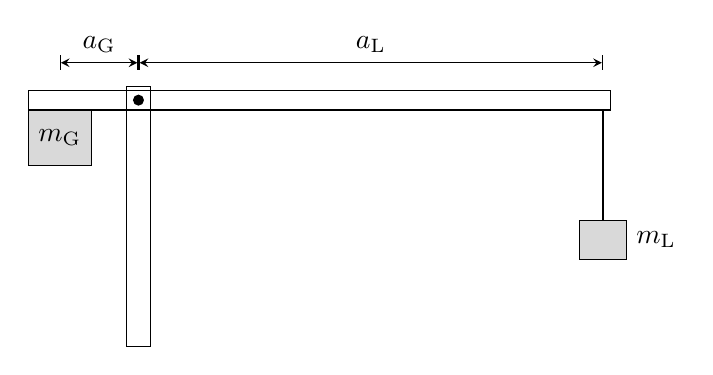
\begin{tikzpicture}[>=stealth]
 \draw (-0.15,-3) rectangle (0.15,0.3);
 \draw (-1.4,0) rectangle (6,0.25);
 \fill (0,0.125) circle (0.07);
 \draw[fill=gray!30] (-1.4,0) rectangle (-0.6,-0.7);
 \node at (-1.0,-0.35) {$m_\mathrm{G}$};
 \draw (5.9,0) -- (5.9,-1.4);
 \draw[fill=gray!30] (5.6,-1.4) rectangle (6.2,-1.9);
 \node[right] at (6.2,-1.65) {$m_\mathrm{L}$};
 \draw[|<->|] (-1.0,0.6) -- (0,0.6) node[midway, above] {$a_\mathrm{G}$};
 \draw[|<->|] (0,0.6) -- (5.9,0.6) node[midway, above] {$a_\mathrm{L}$};
\end{tikzpicture}
\end{center}

Die Drehachse ist der Kranturm. Hängt die Last ganz aussen am Ausleger ($a_\mathrm{L} = \aKrO$), müssen sich die Drehmomente der Gewichtskräfte von Last und Gegengewicht ($a_\mathrm{G} = \bKrO$) aufheben (das Gewicht des Auslegers selbst wird vernachlässigt):
\begin{align}
 m_\mathrm{L}\,g\cdot a_\mathrm{L} &= m_\mathrm{G}\,g\cdot a_\mathrm{G} \\
 m_\mathrm{L} &= \mLaF = \mKr\cdot\frac{\bKr}{\aKr} = \mLa \approx \result{\mLatP{0}{2}}
\end{align}
